Central question for macro and labor: 

\underline{What determines the level of employment and unemployment in the economy?}

In neoclassical model, theoretically cannot deal with unemployment,
because there is no involuntary unemployment.
\begin{enumerate}
    \item Given prices, some agents optimally choose to work zero hours.
    \item There is supply and demand only; demand determined by
    technology or by demand for output; supply driven by inter- or
    intratemporal substitution
    \item There can be under-employment due to wage stickiness, but
    there is no unemployment in equilibrium
\end{enumerate}

\section{Some facts about the labor market}

\begin{itemize}
    \item unemployment is a persistent phenomenon
    \item large flows of workers between employment, unemployment
    and non-participation states
    \item $\Delta u = \text{inflow} - \text{outflow}$
    \item employed workers often change jobs - with a wage gain or
    wage reduction
\end{itemize}

\subsection{How should we model labor friction?}

\begin{itemize}
    \item incentive problems, efficiency wages
    \item wage rigidity, bargaining, non-market clearign prices
    \item search Frictions
\end{itemize}

\begin{definition}[Search and matching]
    \

    It is costly process for workers (firms) to find the right jobs (workers)
\end{definition}

\subsubsection{Facts about job flows}

\begin{enumerate}
    \item job creation is mildly pro-cyclical
    \item job destruction is strongly counter-cyclical
    \item job destruction leads job creation,
    it is the driving force of the business cycle - especially in
    economies with flexible labor markets
    \item job creation seems to be the main cause of long-run changes
    in unemployment
    \item worker turnover about three times as large as job turnover
    \item worker quits are strongly pro-cyclical $\Leftrightarrow$
    offset by the counter-cyclical job destruction rate recession
    $\rightarrow$ job destruction increases
    $\rightarrow$ voluntary quitting decreases
    $\Rightarrow$ inflow to unemployment increases, but less
    \item unemployment changes driven mainly by the outflow from
    unemployment
    \item in monthly data: employment $\leftrightarrow$ non-participation flows
    $\approx$ employment $\leftrightarrow$ unemployment flows
\end{enumerate}

\section{A simple model of unemployment}

(Shimer’s exercise)Let the unemployment rate at period $t$ be $u_t$,
the change in the unemployment rate is
\[u_{t+1} - u_t = s_t(1-u_t) - f_t u_t\]
where $s_t$ is the job separation rate(probability of employed workers move into unemployment), 
$f_t$ is the job finding rate.
We ignore exit from the labor force, and entry from out of labor
force.

Denote average rates by:
\[\bar{s} = \frac{1}{T}\sum_{t=1}^T s_t, \quad \bar{f} = \frac{1}{T} \sum_{t=1}^{T} f_t \]

Compare the actual unemployment rate with
\begin{enumerate}
    \item A hypothetical unemployment rate constructed using the
    average (a constant) separation rate:
    \[u_{t+1} - u_t = \bar{s}(1-u_t) - f_t u_t\]
    \item A hypothetical unemployment rate constructed using the
    average (a constant) job finding rate:
    \[u_{t+1} - u_t = s_t(1-u_t) - \bar{f} u_t\]
\end{enumerate}

\subsection{Lessons from Shimer’s exercise}
\begin{itemize}
    \item separation rate not so important in the evolution of
    unemployment
    \item job finding rate is a more important determinant of
    unemployment
\end{itemize}

\underline{Why?}

separation rates do increase during recessions
BUT the job finding rate is high in the US, even during
recessions, even if more workers get laid off, they find a job quickly $\rightarrow$
job separation rate not so important.

\section{Search and matching models}

\subsection{First generation search models (PE, McCall)}
Let's start right away with continuous time.

Assuming workers start out unemployed, receive unemployment benefits $b\cdot \delta t$in every infinitesimal time interval $\delta t$.

Job offers arrive according to a Poisson process with rate $a>0$, i.e.
in each period of length $\delta t$ a worker receives $n = 0, 1, 2, \cdots$ offers with probability $a(n, \delta t)$,
where
\[a(n, \delta t) = \frac{(a \delta t)^n}{n!} e^{a \delta t} \]
and the number of offers is independent across time.

\begin{remark}
    \

    Assume a constant discount rate rConstant discount rate $r$ 
    and value function of unemployed worker $U$.
    
    If you stay unemployed, you can never be worse off than $rU$, 
    so unless someone pays at least this, you won’t start working
\end{remark}

\section{Second-generation model(Mortensen and Pissarides, 1994)}

\subsection{Two-sided matching}
To close the one-sided search model, to derive a proper equilibrium
of the economy, we need to
\begin{enumerate}
    \item Make arrival date $a$ endogenous, to specify decision of firms whether or not to offer jobs
    \item ensure that employment is not an absorbing state, exogenous job destruction, at rate $\lambda$
    
    interpretation: negative shocks arrive to existing matches, that destroy the match
    \item the wage is the result of bargaining between the matched
    worker and firm
\end{enumerate}

\subsection{The matching function}

\subsubsection{Key assumption}
The aggregate flow depends on an aggregate matching function.

Vacancy posting is a (risky) investment for firms: it is costly to post a
vacancy, but if firms successfully hire workers, they can enjoy the profit arising from produc-
tion in the future. Unemployed workers search for firms to work for. The matching process
between firms (vacancies) and unemployed workers is summarized by the \textit{matching function}:
\[m = m(u, v)\]
where $m(\cdot)$ is increasing in both terms and exhibits constant returns to scale.


\subsection{The matching function}
The empirical literature (Petrongolo \& Pissarides 2001) found
that a Cobb-Douglas function matches the data well:
\[m = Au^{\eta}v^{1-\eta} \]
where usually $\eta=0.5$.

Job matching is pairwise: $m = au = qv$, where:
arrival rate of workers to vacant jobs 
\[q = \frac{m(u, v)}{v} = m\left(\frac{u}{v}, 1\right) = m(\theta^{-1}, 1) = q(\theta)\]
where $q$ is a decreasing function of $\theta $, and the elasticity of $q$ w.r.t $\theta $ is $\pd{q}{\theta} \frac{\theta}{q} = -\eta \in (-1,0)$.

arrival rate of jobs to workers
\[a = \frac{m(u, v)}{u} = m\left(1, \frac{v}{u}\right) = a(\theta) = \theta q(\theta)\]

$\theta =\frac{u}{v}$ is a measure of \textit{market tightness}.

$u$ is a state, $v$ is the firm's control, which drives unemployment.

However, probably both firms and workers ignore their effect
on $\theta$ when they make their search choices$ \rightarrow$ \textbf{search externalities}.

\begin{figure}[!htbp]
    \centering
    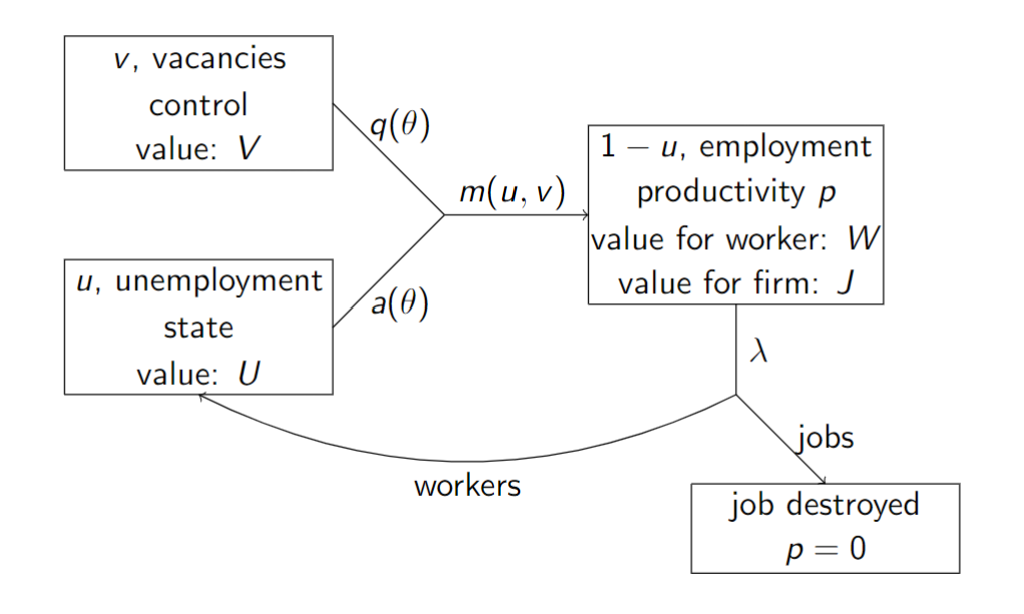
\includegraphics[width=0.8\textwidth]{figures/matchsearching.png}
    \caption{Match and searching model}
\end{figure}

\subsection{Value of vacancis and jobs}
We define
\begin{itemize}
    \item $V$: value of a vacancy
    \item $J$: value of a job
\end{itemize}

A job is an asset owned by the firm, and its value is determined by arbitrage equations:
\begin{align*}
    rV &= -pc + q(\theta)(J-V) \\
    rJ &= p - w - \lambda J
\end{align*}
where $r$ is the discount rate, $p$ is the value of product, 
$pc$ is the cost of mainting a vacancy, $w$ is the wage, 
$\lambda$ is the job destruction rate.

Firm creates a job vacancy when there are gains from entering the
market and there is free entry.

Zero profits $V = 0$ means that $J = \frac{pc}{q(\theta)}$.

$\frac{1}{q(\theta)}$ is the expected duration of a vacancy.

$\frac{pc}{q(\theta)}$ is the expected to tal cost of finding a worker.

\subsection{Job creation}
Thevalue of a filled job is: 
\[J = \frac{p-w}{r + \lambda}\]

\begin{note}
    \

    For the firm to accept a wage $w$, the value of the job must be at least $w$($p \geq w$).
\end{note}

Combine the two functions of the value of filled jobs: 
\[\underset{\text{profit flow}}{\underbrace{p-w}} - \underset{\text{expected cost of finding a worker}}{\underbrace{\frac{(r+\lambda)pc}{q(\theta)}}} = 0\]

\underline{Job creation condition:} generalization of the labor demand
condition, downward sloping in the $\theta - w$ space.

\subsection{Wage determination}
Wages are determined through a process of bargaining between
firm and worker. 

Using Nash bargaining, each party gets outside option plus a
fraction, $\beta $ for worker , $1-\beta $ for firm, of the difference
between total surplus and outside options. 

This process yields a wage equation:
\[w = (1-\beta)z + \beta p(1 + c \theta) \]
which is:
\begin{itemize}
    \item increasing in the worker outside option $z$
    \item increasing in the worker marginal product $p$
    \item increasing in the bargaining power of the worker $\beta$
    \item increasing in the market tightness $\theta$
\end{itemize}

\begin{figure}[!htbp]
    \centering
    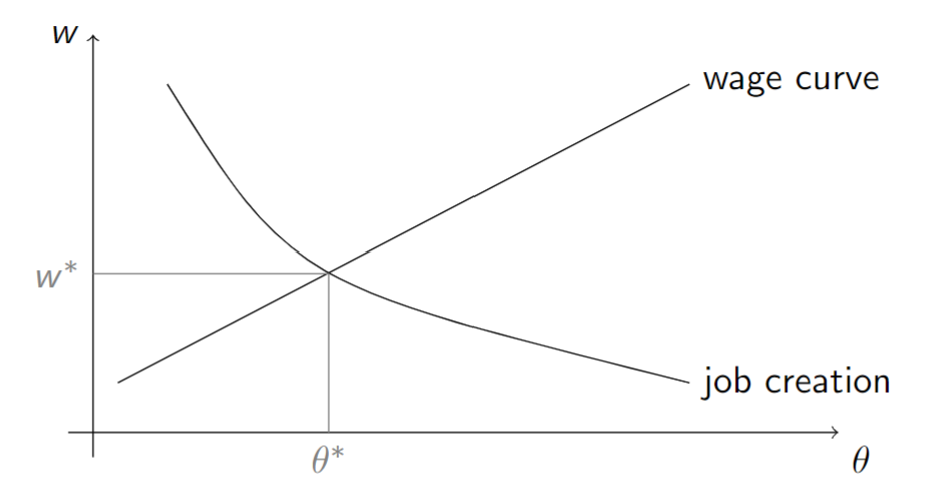
\includegraphics[width=0.8\textwidth]{figures/wagejobeq.png}
    \caption{Equilibrium wages and market tightness}
\end{figure}

In this economy, the equilibrium is a path for

\underline{The controls:}
\begin{itemize}
  \item Wages -- from the wage equation: $J \geq 0, W \geq U$
  \item Job vacancies (or tightness) -- from job creation $V = 0$
\end{itemize}

\underline{The state:}
\begin{itemize}
  \item Employment -- \textit{condition for the evolution of unemployment}
\end{itemize}
\[
\dot{u} = \lambda (1 - u) - m(u, v) = \lambda - (\lambda + \theta q(\theta))u
\]
Given $\theta^*$, this has a unique stable solution, the \textit{natural rate of unemployment}:
\[
u = \frac{\lambda}{\lambda + \theta^* q(\theta^*)}
\]
The above is the \textit{Beveridge curve}.

\begin{figure}[!htbp]
    \centering
    \begin{minipage}[b]{0.45\textwidth}
        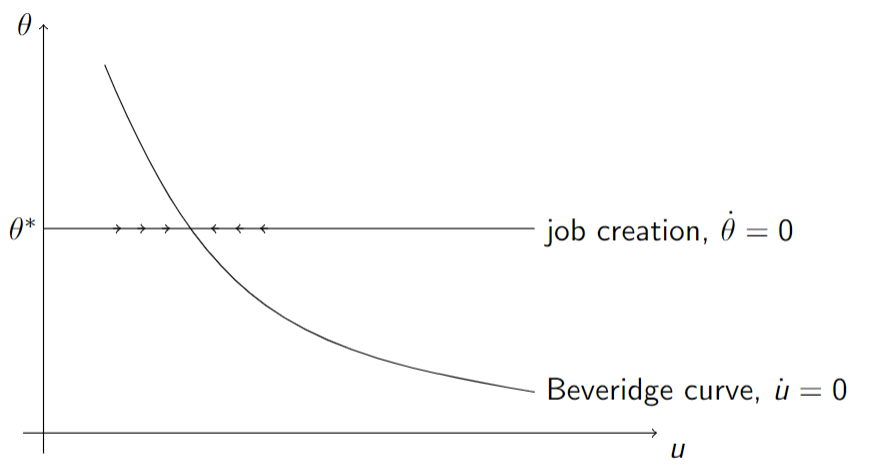
\includegraphics[width=0.8\textwidth]{figures/constantjobcreation.png}
        \caption{Constant Job Creation Beveridge curve}
    \end{minipage}
    \begin{minipage}[b]{0.4\textwidth}
        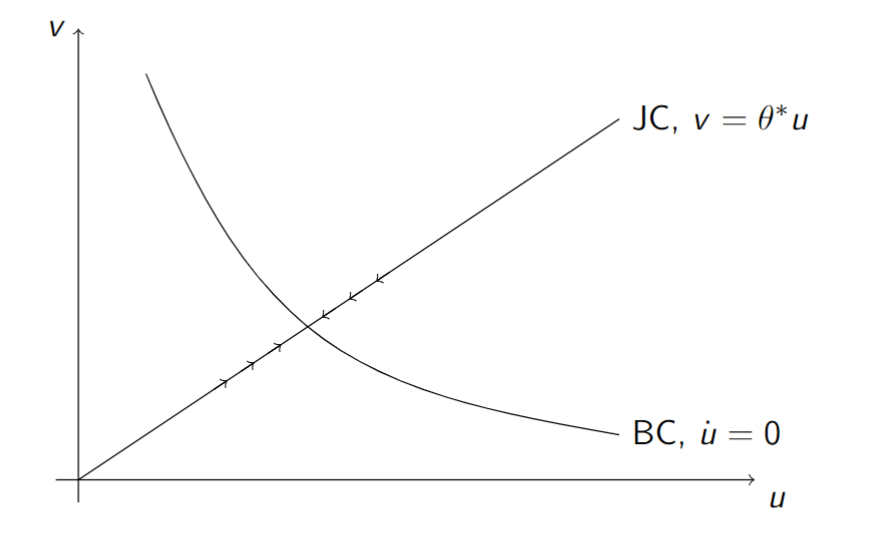
\includegraphics[width=0.8\textwidth]{figures/beveragecurve.png}
        \caption{Beveridge curve}
    \end{minipage}
\end{figure}

Assuming a permanent increase in $A(MPL)$, the job-wage curve would shift up right,

For the Beveridge curve, because $u$ cannot
jump, $v$ immediately decreases so that $\frac{v}{u}$ becomes the new value at point $B$,
After that, the economy gradually converges to the new steady state of $C$ on the new job creation curve.
\begin{figure}[!htbp]
    \centering
    \begin{minipage}[b]{0.45\textwidth}
        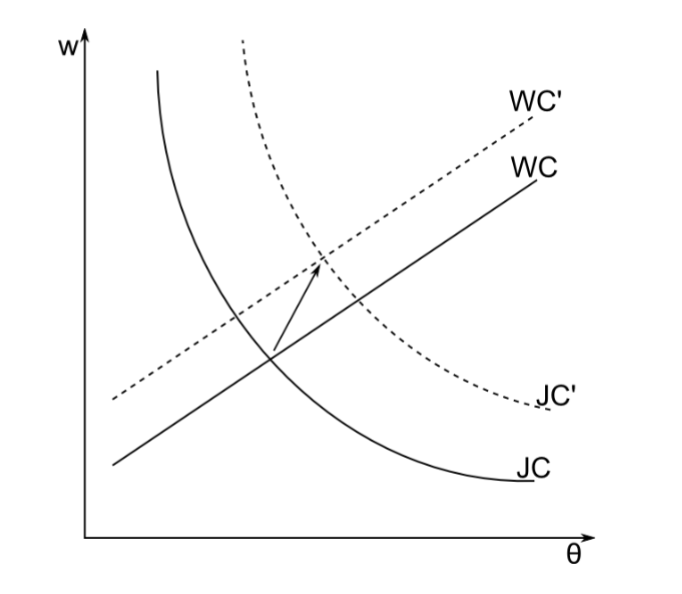
\includegraphics[width=0.8\textwidth]{figures/newjobwage.png}
        \caption{Shift in job-wage curve}
    \end{minipage}
    \begin{minipage}[b]{0.45\textwidth}
        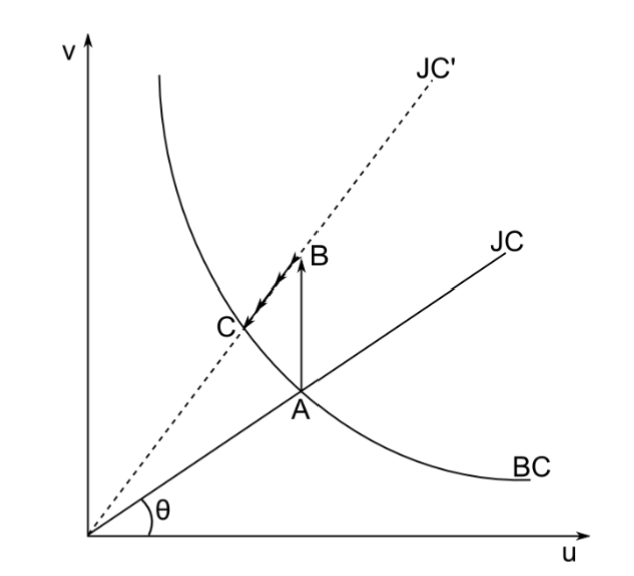
\includegraphics[width=0.8\textwidth]{figures/BCshift.png}
        \caption{Shift in Beveridge curve} 
    \end{minipage}
\end{figure}

For a temporary positive TFP shock, JC curve will rotate back to the original position over time,
and respons eto $u$ would be U-shaped.

If unemployment flow utility $b$ is high enough, elasticity of wage is low.

\subsection{The unemployment volatility puzzle}

The mpirical implementations of this model
\begin{enumerate}
    \item can match contemporaneous correlations between
    unemployment and vacancies
    \item \textcolor{blue}{cannot match the volatility of unemployment, vacancies,
    tightness, job finding rate (no amplification)}
    \item \textcolor{blue}{cannot match the correlations with labor productivity}
\end{enumerate}
This discrepancy is often referred to as the \textit{unemployment
volatility puzzle} or the labor market volatility puzzle 
(or the \textcolor{blue}{\textbf{Shimer puzzle}}, after Shimer(2005)).

\begin{remark}[Reasons for the Shimer's puzzle]
    \

    Intuitively, there are two reasons, corresponding to benefits and 
    costs of hiring, for the quantitatively small response. 

    First, the benefit of hiring a worker is procyclical, but the magnitude is not large. 
    One reason is that the wage increases in booms, and it weakens the 
    response of profit to the productivity shock. 

    Second, the cost of hiring a worker moves together with $\theta$. 
    In booms, $\theta$ increases, and this increase in cost 
    restricts the firm’s response to a positive productivity shock.
\end{remark}

\underline{What happens after a TFP shock?}
\begin{itemize}
    \item Wage increases, but not as much as the MPL
    \item Hence firms want to increase employment. More vacancies
    get posted.
    \item Over time, this reduces the unemployment rate.
\end{itemize}
\underline{Hence}:
\begin{itemize}
    \item Since the intensive margin of labor supply is fixed, higher
    wages do not increase labor supply
    \item Any effect on $u$ must go through vacancy posting
    \item But wage is too elastic: MPL - $w$ increases by too little, few
    vacancies are being posted
\end{itemize}

\subsubsection{Possible solutions}
\begin{itemize}
    \item Sticky wages;
    \item Make unemployment not a big deal, low vacancy posting costs;
    \item Fixed costs for vacancy posting.
\end{itemize}